\documentclass{article}
\usepackage[utf8]{inputenc}
\usepackage{graphicx}
\usepackage{float}

\title{Explanation}
\author{Pawan Mali }
\date{June 2026}

\begin{document}
\maketitle
\section{Provided Repository structure Explanation}

I analyzed the local folder. It contains two ROS 2 workspaces:

\begin{figure}[H]
    \centering
    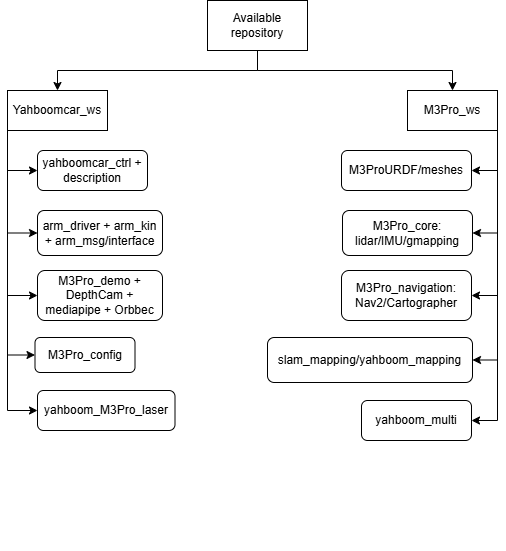
\includegraphics[width=0.9\textwidth]{Img/Repo_Downloaded.png}
    \caption{Overview of the downloaded repository structure}
    \label{fig:repo_structure}
\end{figure}

\subsection{yahboomcar\_ws/src}

\begin{itemize}
    \item \textbf{yahboomcar\_ctrl}: Keyboard and joystick teleoperation. Important files include \texttt{yahboom\_keyboard.py} and \texttt{yahboom\_joy\_M3Pro.py}.
    
    \item \textbf{yahboom\_M3Pro\_description}: Contains the robot URDF, meshes, and RViz model display files.
    
    \item \textbf{M3Pro\_config}: MoveIt2 configuration package containing arm planning settings and fake \texttt{ros2\_control} configuration.
    
    \item \textbf{M3Pro\_demo}: Includes computer vision and manipulation demonstrations such as AprilTag detection, color tracking, KCF tracking, grasping, and line-following.
    
    \item \textbf{yahboom\_M3Pro\_laser}: Lidar-based applications including obstacle avoidance, obstacle warning, and target tracking.
    
    \item \textbf{yahboom\_M3Pro\_DepthCam}: Depth camera examples including distance measurement, depth-color visualization, and edge detection.
    
    \item \textbf{OrbbecSDK\_ROS2}: ROS 2 driver package for Orbbec/Dabai depth cameras.
    
    \item \textbf{arm\_interface, arm\_msgs}: Custom messages and services used for robotic arm communication.
    
    \item \textbf{arm\_kin}: Forward and inverse kinematics services implemented using KDL.
    
    \item \textbf{arm\_driver}: Serial communication driver for the robotic arm using the Rosmaster library.
\end{itemize}

\subsection{M3Pro\_ws/src}

\begin{itemize}
    \item \textbf{M3Pro}: Robot URDF, meshes, and model display launch files.
    
    \item \textbf{M3Pro\_core}: Core robot packages including laser merging, laser filtering, IMU filtering, and GMapping support.
    
    \item \textbf{M3Pro\_navigation}: Navigation stack configuration including Nav2, Cartographer localization, and RViz navigation setups.
    
    \item \textbf{slam\_mapping, yahboom\_mapping}: Packages used for SLAM and map generation/saving.
    
    \item \textbf{ekf\_bringup}: Robot localization package that fuses \texttt{/odom\_raw} and \texttt{/imu/data} using an Extended Kalman Filter (EKF).
    
    \item \textbf{calibration}: Linear and angular calibration utilities based on \texttt{/cmd\_vel} and TF data.
    
    \item \textbf{yahboom\_multi}: Multi-robot navigation and coordination configurations.
    
    \item \textbf{patrol}: Laser-based autonomous patrol behavior implementation.
    
    \item \textbf{largemodel, largemodel\_arm}: AI, voice interaction, and computer vision application examples.
\end{itemize}

\end{document}

